\section{并行计算中的负载均衡化策略}
%并行计算框架十分重要
随着当下信息技术的快速发展,科学计算产出的数据体量快速提升。与此同时,针对复杂数据本身所定义的计算任务也逐渐变得更加复杂。针对这一类大规模数据的复杂任务,并行计算的模式成为了一种十分行之有效的解决方案。并行计算指同时使用多种计算资源解决计算问题的过程,它的基本思想是用多个处理器来协同求解同一问题,即将被求解的问题分解成若干个部分,各部分均由一个独立的处理器进行计算。这可以大大提升科学计算的效率。近年来,随着高性能计算技术的发展,研究者可以更多地利用超级计算机或者并行计算集群等强大的计算资源来进行并行计算,十分有效地提升了计算结果产出的效率。

%通用并行计算框架中负载均衡问题的重要性
在并行计算的过程中,负载均衡问题显得尤为重要,需要设计精细的任务分配和调度策略,使得在并行计算的整个过程中,每个计算节点都始终被分配有较为均衡的任务量,才能最大化地利用计算资源,达到效率的最优化。如果没有较好的基于负载均衡的资源调度算法,由于初始算法的分配的不均衡和计算过程中的随机演化,负载不均衡问题时常会发生。由于计算任务本身的特性的制约,负载均衡问题也成为提升并行计算效率中的一个瓶颈所在。

%负载均衡算法简单分类
针对负载均衡的问题的解决方案通常分为静态负载均衡算法和动态负载均衡算法,不同的算法针对不同的任务场景可以高效的提升并行计算的效率。静态的负载均衡算法通常根据数据或任务的的基本特性,初始地决定任务分配和资源调度的方式,在后续的并行计算过程中不再进行后续的调度方式。这要求这一类静态负载均衡算法需要有效地预估整个并行计算过程中各个计算节点的负载,统筹兼顾全局和单个轮次,有效地帮助计算效率地提升。相对于静态负载均衡算法,动态负载均衡算法相对更加灵活有效。动态负载均衡算法不仅仅考虑初始的数据和任务特性,而是同时考虑系统的实时的状态信息决定系统负载的分配,能够适应并行计算过程中的演化,高效的实现实现系统的负载均衡。动态负载均衡算法更加复杂,因而需要考虑更多的系统状态信息,需要更多的计算资源进行处理。对于系统的负载均衡问题的处理本身就需要达成成一种平衡,即预处理代价和等待以及负载平衡后收益的权衡,需要仔细的计算和考量。相对于静态负载平衡算法,动态负载平衡算法对于整个粒子追踪的过程施加了更多的干预,因而引入了更多的预处理代价,同时使得整个过程更加复杂多变,难以预测和掌控。对于上述两种算法的使用与选择,则需要根据具体的应用场景具体分析,依据数据和任务的演化和特征,合理设计任务的调度算法,才能使得负载均衡对于整个并行计算过程的效率有较大的提升。

\subsection{流场可视化中的针对负载均衡问题的挑战}
%引入流场可视化中的并行计算任务
在科学可视化中针对大规模流场的可视化任务中,基于粒子追踪的流场可视化需要从原始数据出发生成场线。这个过程计算复杂,计算量大,而且在一些需要追踪大规模密集撒种的粒子的应用中,最后的场线规模往往比原始数据更大(甚至可能达到几个数量级的差距)。
此外,随着现代科技和计算技术的高速发展,流场数据的数据量正以几何级数的速度增长。流场本身和相关的分析任务也呈现出越来越复杂的趋势。
特别地,在一些诸如线积分卷积(line integral convolution, LIC)\parencite{CabralL93,ShenK97}、
基于有限时间李雅普诺夫指数(finite-time Lyapunov exponents, FTLE)计算的拉格朗日拟序结构(Lagrangian coherent structures, LCS)
提取\parencite{Haller2001,GarthGTH07}以及流场曲面(flow surface)计算\parencite{EdmundsLCMZW12}、
源汇查询(source-destination queries)\parencite{KendallWAPHE11}等基于场线的应用中,往往需要进行复杂的粒子追踪计算。
现实应用中单台处理机由于内存和计算能力等的限制,很难满足这种大规模粒子追踪的计算需求。
而早前研究者所使用的核外(out-of-core)技术\parencite{silva2002out,BruckschenKHJ01,EllsworthGM04}
因其I/O瓶颈在大规模流场数据中也变得越来越不适用。

%流场可视化中采用并行计算的优势
而通过采用并行计算的模式,将工作负载分布到成百上千上万甚至更多的计算节点单元(本文所提到的每个节点单元一般对应一个计算进程),由这些节点单元协作计算大规模粒子的轨迹,粒子追踪的效率会大大提高。
这也使得并行粒子追踪成为了目前基于场线的大规模流场可视化的主流趋势。

%流场可视化中采用并行计算的方法 任务/数据并行
原始数据和输入粒子经过划分,每个进程单元都会分配到一定的数据或粒子,并进行粒子追踪计算。
按照划分和分配对象的不同,并行粒子追踪主要分为两类。
一类以粒子为对象,称为任务并行(每个粒子可看成是一个任务),
每个进程分配到的是输入粒子的一部分,
数据通常会在追踪计算过程中被按需载入。
在并行粒子追踪过程中,进程各自对所负责的粒子进行追踪计算。
另一类以数据为对象,称为数据并行,其将数据划分为若干数据块,
每个进程分配到其中的一部分,输入粒子按照其初始位置所在数据块也会被分配到不同的进程中,
数据在开始追踪计算前就被载入到各进程内存中。
为了保证每个粒子的追踪能够完成,
在并行粒子追踪过程还会周期性地发生数据的移动(针对任务并行,从外存移动到内存或者在进程之间移动)
或者粒子的交换(针对数据并行,在进程之间交换)。
当所有进程完成各自的粒子追踪计算,整个并行计算过程会停止。
经过计算得到的场线会被用于对流场的可视化和分析。


% 流场可视化中负载均衡的问题
但是,不同于其他领域的并行计算,粒子追踪的并行化本身存在着比较复杂的问题。 
在进行粒子追踪过程中,粒子的运行时间也难以预测。
粒子追踪的自然终止条件一般是粒子穿出数据域的边界,或者遇到临界点等速度为零的地方,
在此之前,如果没有人为设定终止条件,粒子会一直在数据场内运动。给定一个初始粒子,粒子会在什么时候停止追踪计算难以预测,其积分步数难以确定,因此负载也难以预测。这样,对粒子的初始划分很难保证进程的负载均衡。这些问题实际上也是并行计算中的经典问题,但是粒子追踪的特性大大加重了这些问题的严重性。

\subsection{任务并行的流场可视化中的针对负载均衡问题的经典解决方案}
% 流场可视化中负载均衡的问题的解决方案
% 针对任务并行
在任务并行中,由于粒子的完成时间不同且难以预测,
初始的粒子划分和分配难以使每个进程获得均衡的负载。
当前的研究工作主要使用一些动态负载调整方法,
即在粒子追踪过程中通过动态地重新分配任务(粒子)而平衡各进程工作负载。
已有方法中,动态任务重分配算法主要分为两类,主要包括工作窃取(work stealing)和工作请求(work requesting)。
其基本思想都是当某一个工作进程完成所负责的任务时,从其他繁忙进程处转移一部分任务给该进程。这种负载状态的监听和任务的调度过程是通过一个主进程来完成的。在任务转移的过程中,数据也需要随之一同被分配,以满足粒子追踪的要求。因而实际上,这里面涉及到的也是数据的动态调度管理。不过,虽然不需要静态的数据预处理操作,这些方法因为需要专门的进程(或线程)进行调度,会带来较大的通信开销,限制了其可扩展性。
而且,在并行粒子追踪的动态过程中进行干预操作,这一操作带来的性能增益可能会被其带来的额外开销抵消掉,甚至会带来负面的影响。

基于工作窃取的算法中较为典型的工作是一种分区全局地址空间(PGAS, Partitioned Global Address Space)建模下的动态任务重分配算法\parencite{DinanLSKN09}。在该算法的指导下,每一个计算进程会维护一个双向队列来保存其即将执行的任务。当每一个进程需要执行任务时,其从队首获得其即将执行的任务信息。当一个进程处于空闲状态时,其将开始进行一种“窃取”的操作。进行“窃取”的进程首先需要从其他的进程中选择一个“受害者”进程。选取的策略存在多种,但已有工作已经证明了随机的选取方式为最优选取方式\parencite{blumofe1999scheduling}。一旦“受害者”进程被选中后,进行“窃取”的进程首先从“受害者”进程中获取元数据来确认是否他们有可以获取的工作任务。如果确认存在可以“窃取”的任务,则“受害者”进程维护的任务队列会被锁定,“窃取”任务的进程则会将多个任务从受害者进程的维护的任务队列的尾部将任务转移给自己,转移的任务数量可以是一个或多个。如果受害者进程没有多余的任务可供“窃取”,则进行“窃取”操作的进程再一次随机的选择一个新的“受害者”进程,并重复这一操作,直到获取了可以执行的任务亦或者是其检测到了全局完成的信号。图\ref{fig:loadbalance:workstealing}展示了基于上述流程总结的算法伪代码。

\begin{figure}[!tb]
%\setlength{\abovecaptionskip}{0.05cm} 
%\setlength{\belowcaptionskip}{-0.20cm}
  \centering
  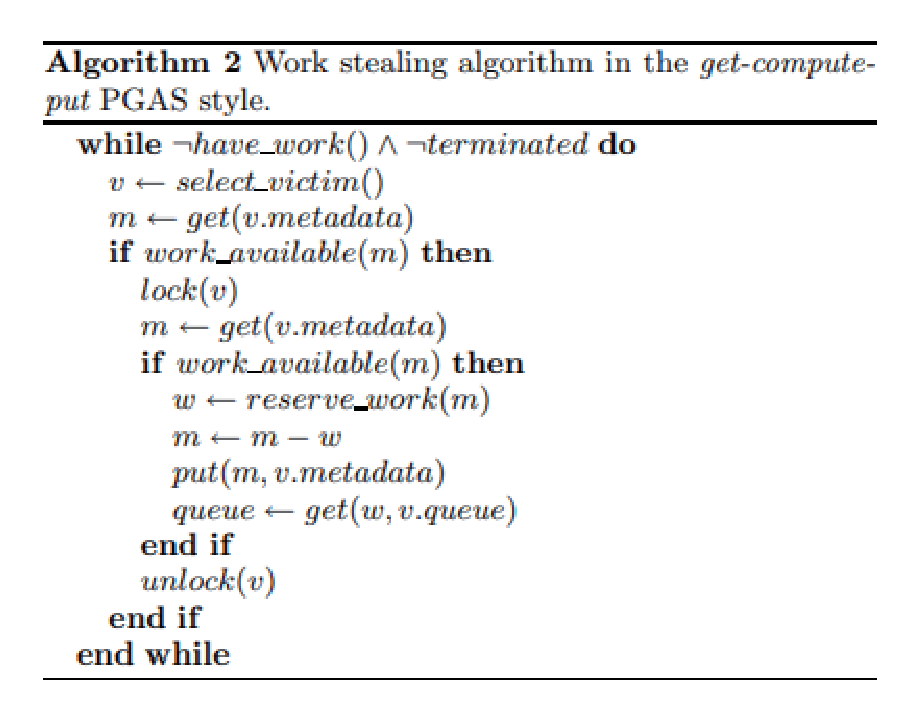
\includegraphics[width=0.7\linewidth,keepaspectratio]{image/loadbalance/PGAS_workstealing.eps}
  \caption{
    分区全局地址空间建模下的基于工作窃取的动态任务重分配算法\parencite{DinanLSKN09}。
 }
\label{fig:loadbalance:workstealing}
\end{figure}

基于上述方式的动态任务重分配算法可以灵活地适用于多种流场可视化应用,并基于MPI消息通信的并行框架可以带来有效地实现。俄亥俄州立大学的可视化小组针对流场可视化中的流面绘制计算过程就施加了基于工作窃取的算法以解决并行计算中的负载均衡问题\parencite{LuSP14}。其基本算法如图\ref{fig:loadbalance:workstealing_mpi}所示。

\begin{figure}[!tb]
%\setlength{\abovecaptionskip}{0.05cm} 
%\setlength{\belowcaptionskip}{-0.20cm}
  \centering
  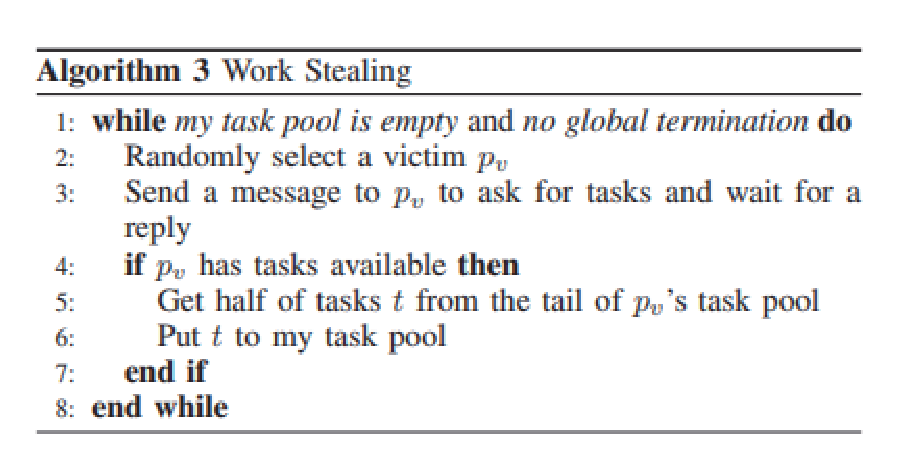
\includegraphics[width=0.7\linewidth,keepaspectratio]{image/loadbalance/streamline_workstealing.eps}
  \caption{
    基于MPI并行框架下基于工作窃取的动态任务重分配算法\parencite{LuSP14}。
 }
\label{fig:loadbalance:workstealing_mpi}
\end{figure}

基于工作请求的算法与基于工作窃取的算法原理相似。不同于基于工作窃取的算法中多个工作进程之间直接进行通信,并转移工作负载和对应的数据,基于工作请求的算法将不同进程根据其不同职责划分为工作进程和监管者进程两类\parencite{MullerCHG13}。算法之所以进行上述的改良是因为试图进行“窃取”操作的进程与“受害者”进程之间试图建立通信时,受害者进程可能处于计算任务的状态而导致长时间难以回应,继而空闲进程需要长时间才能获取分担其他进程的任务。在基于工作请求的算法中,工作进程负责数据I/O和粒子追踪积分计算,当其完成其任务队列中的所有任务时,则向监管者进程发出工作需求申请,监管者进程收到工作需求申请后,若其持有未完成的工作任务,则将半数的任务递交给提交该申请的工作进程。当监管者进程发现其持有的工作任务均被派出,则同样随机选取一个“受害者”进程并向其请求一部分任务。整个过程中,监管者进程起到了调度者的角色,减少了与工作进程通信的次数,减少了等待的时间,同时使得全局的通信模式更加合理。其基本算法如图\ref{fig:loadbalance:workrequesting}所示。

\begin{figure}[!tb]
%\setlength{\abovecaptionskip}{0.05cm} 
%\setlength{\belowcaptionskip}{-0.20cm}
  \centering
  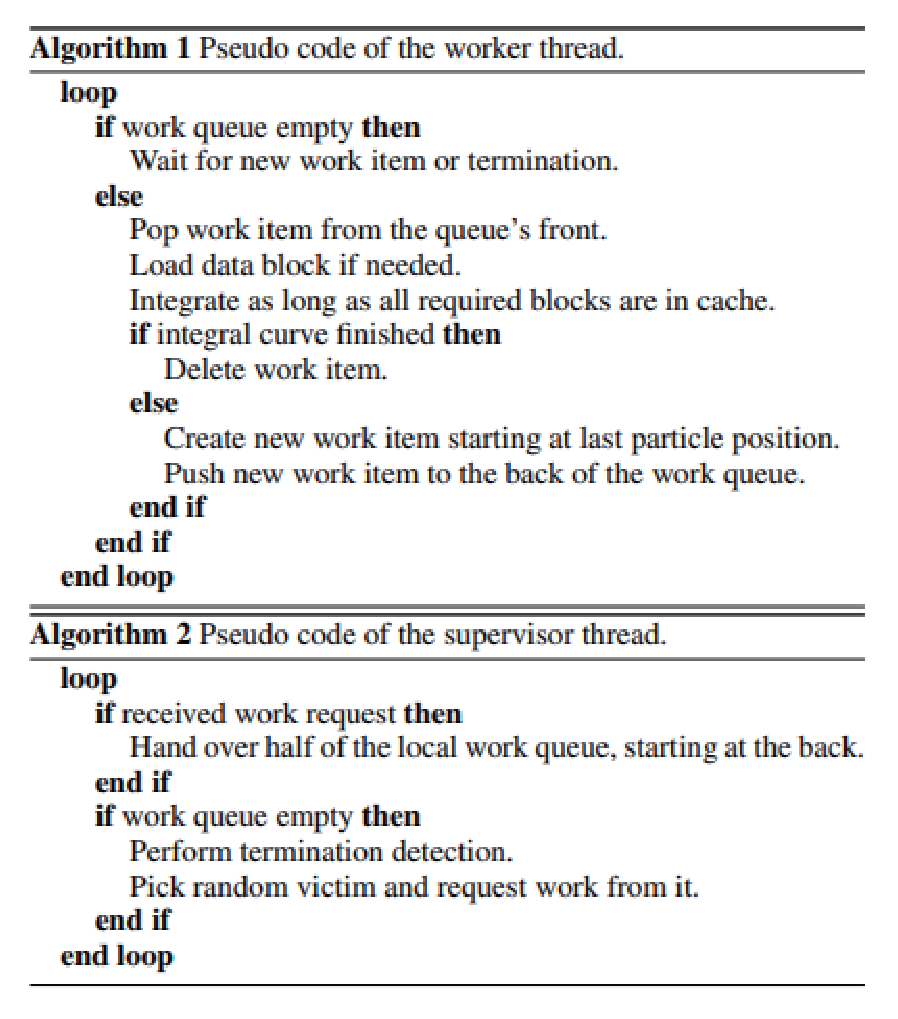
\includegraphics[width=0.8\linewidth,keepaspectratio]{image/loadbalance/workrequesting.eps}
  \caption{
    基于工作请求的动态任务重分配算法\parencite{MullerCHG13}。
 }
\label{fig:loadbalance:workrequesting}
\end{figure}

北京大学可视化与可视分析小组提出了另一种针对任务并行的动态负载平衡的算法\parencite{ZhangGHYP18}。具体的说,其使用基于k-d结构的数据划分管理策略,通过周期性地进行k-d树的分解来尽量均匀地对粒子进行重新分配,从而达到负载均衡的目的。

\begin{figure}[!tb]
%\setlength{\abovecaptionskip}{0.05cm} 
%\setlength{\belowcaptionskip}{-0.3cm}
  \centering
  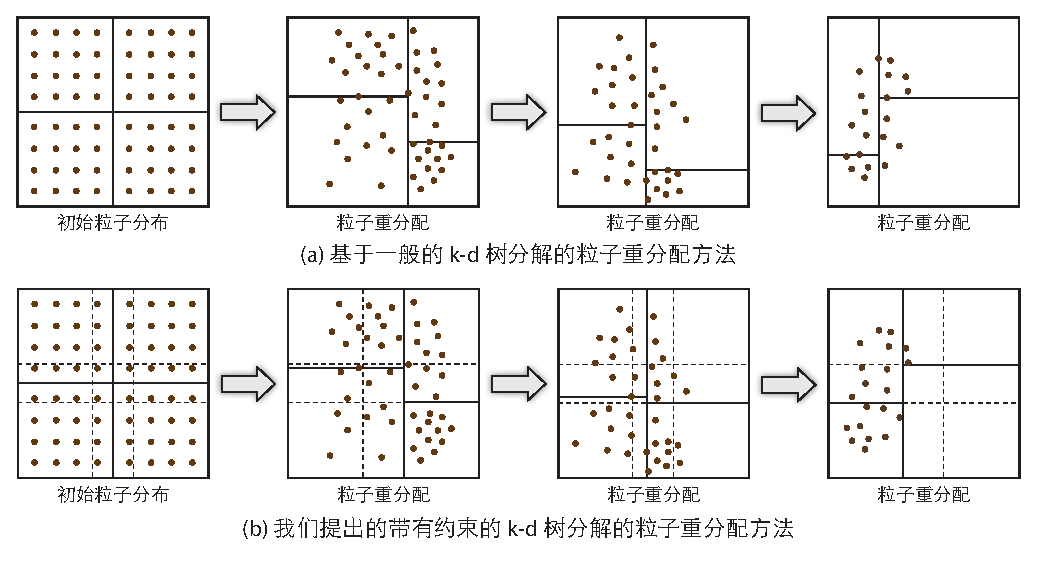
\includegraphics[width=0.99\linewidth]{image/loadbalance/basic-idea}
  \caption{
    基于一般k-d树分解的和新的带有约束的k-d树分解的粒子重分配示例。\parencite{ZhangGHYP18}
    在图(a)和(b)中,实线表示的切分线将粒子尽量划分均匀。
    图(b)中的虚线展示了由ghost层组成的数据重叠区域,其限制了切分线的位置。
  }
  \label{fig:kdtree:basic-idea}
\end{figure}

在该方法中,每个进程被分配到(1)一个静态划分的数据块,
该数据块与其相邻的被分配到其他进程的数据块会产生部分重叠;
(2)一个动态确定的k-d树叶结点,
该结点的范围受到对应数据块的几何约束,用于限制活动的粒子的重分配。
在给定的数据块重叠程度下,该方法可以最大可能地平衡各进程中粒子的数目。
与其他针对并行粒子追踪的负载平衡算法相比,
该方法不进行任何的预先分析,不使用基于流场特性的任何启发,
不对初始粒子种子的分布做任何假设,
在运行期间不移动任何数据块,并且不需要任何主进程进行任务的调度。

\begin{figure}[H]
%\setlength{\abovecaptionskip}{0.05cm} 
%\setlength{\belowcaptionskip}{-0.3cm}
  \centering
  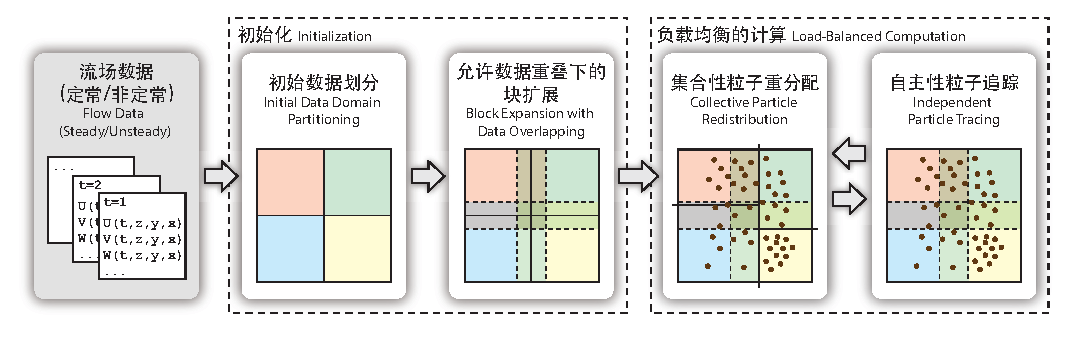
\includegraphics[width=\linewidth,keepaspectratio]{image/loadbalance/workflow_kdtree.eps}
  \caption{
    动态负载平衡方法的工作流程\parencite{ZhangGHYP18}。
    在初始化阶段原始数据首先被划分为块。
    通过增加ghost层,这些块会被扩展,使得在内存限制下与其他块有最大的数据重叠。
    在运行时阶段,集合性粒子重分配和自主性粒子追踪会被轮流执行,以动态地达到负载平衡。
  }
  \label{fig:kdtree:workflow}
\end{figure}

该方法首先对数据块和粒子进行初始化。

{\bf 数据域划分}\quad 算法通过迭代地切分数据域的每个维度来划分输入数据;
数据维度被划分的顺序与k-d树分解的一致。
不失一般性,该方法假定进程数$n$是2的幂(如果不是的话算法也可以根据其素数分解来划分每个维度)。
举例来说,在3D数据中,算法在$x$轴上找到一个位置将数据域均匀划分为两个块,
然后将这两个块的每一个再沿着$y$轴划分成两个块,然后对每一个块再沿着$z$轴划分。
$z$轴之后,下一个划分的维度又是$x$轴。
该过程一直迭代下去,直到数据块的数目等于$n$。此时每个进程可以拥有一个数据块。 数据域划分的结果是得到$n$个无重叠、相等大小、轴对齐的数据块。

{\bf 数据块扩展}\quad 该方法通过在数据块上加上ghost层来最大化块之间的数据重叠。
如图\ref{fig:kdtree:ghost}所示,每个块在所有维度上被扩展,并因此与邻近的块产生数据重叠。
块扩展使得k-d树分解的切平面可以在这个重叠区域内进行切分,其详细介绍会在下节解释。
数据块能够扩展的厚度由进程的可用内存所决定。
在内存可以容纳下整个数据的极端情况下,每个进程保存了完整的数据副本。

{\bf 数据块I/O读取}\quad 该方法并行地载入扩展后的数据块,使得每个进程将其所负责的那一部分数据读取进内存。
并行I/O由BIL(block I/O layer)\parencite{KendallHPLR11}库所实现,
其本质上是使用并行I/O以可扩展的方式来读取扩展后的数据块。

{\bf 粒子初始化}\quad 该方法载入输入粒子并且将它们在不同的进程上进行分布。
每个粒子被分配给"核心"区域(即除去ghost层)包含该粒子的数据块。
\begin{figure}[!tb]
%\setlength{\abovecaptionskip}{0.05cm} 
%\setlength{\belowcaptionskip}{-0.3cm}
  \centering
  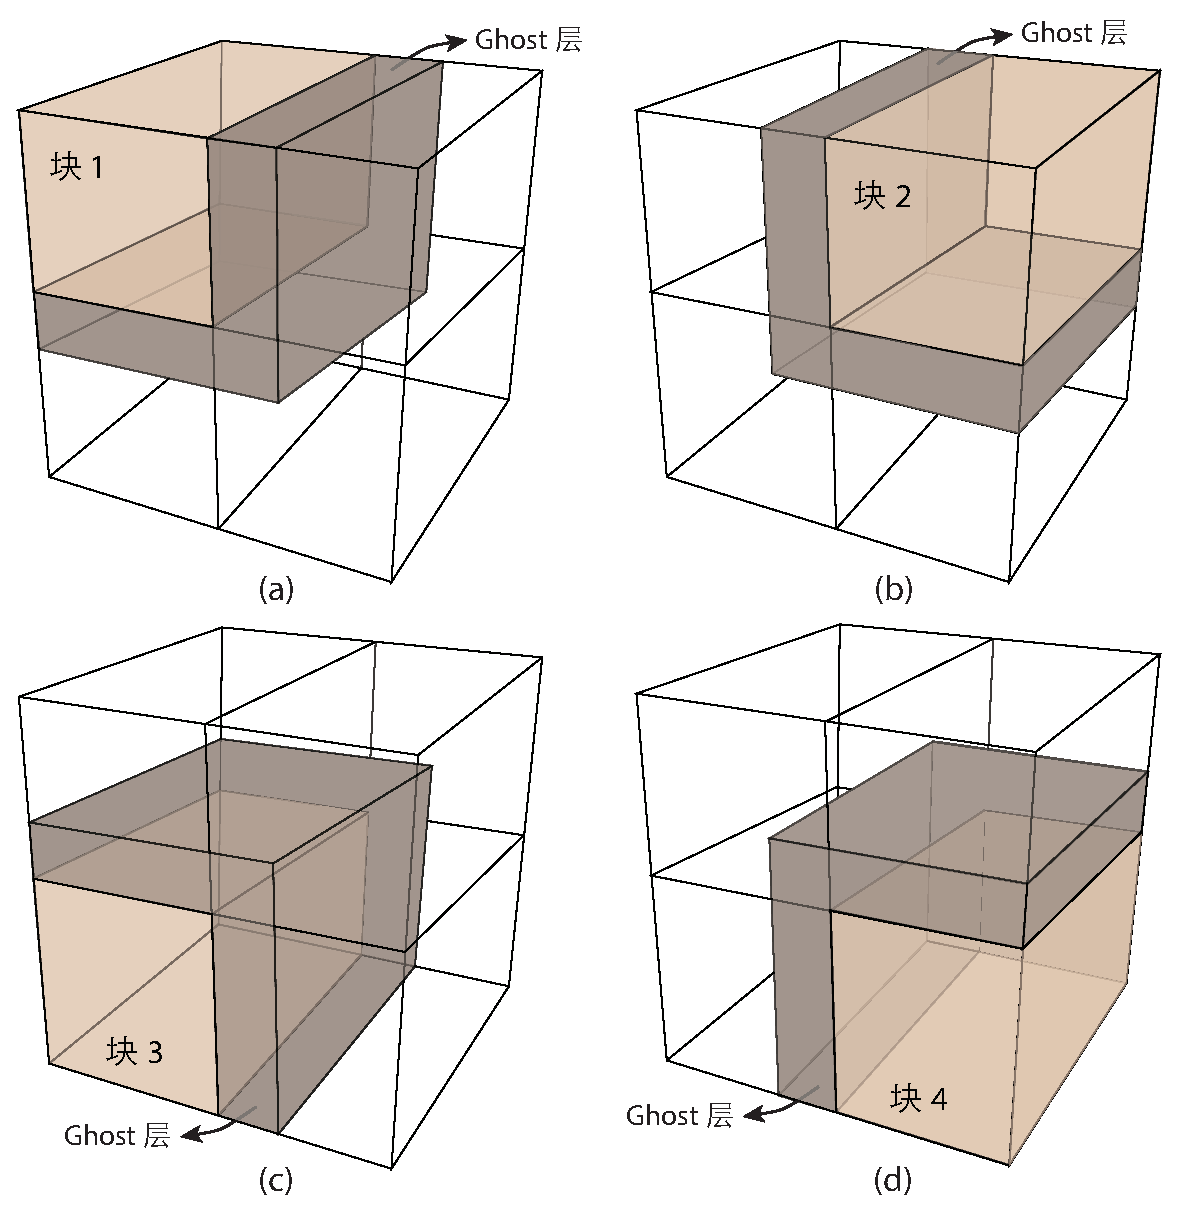
\includegraphics[width=0.6\linewidth]{image/loadbalance/ghost}
  \caption{四个经过扩展的3D数据块划分的示例\parencite{ZhangGHYP18}。}
  \label{fig:kdtree:ghost}
\end{figure}

该算法循环遍历每个维度来划分数据域。
对于每个维度,算法试图找到一个可以均匀切分粒子的轴对齐的中间平面。
如果该平面不在两个相邻数据块的重叠区域之内,则
在重叠区域的两个边界中选择可以尽可能平衡粒子数目的那个边界作为切平面的位置。

该方法重新设计了分布式k-d树分解算法\parencite{MorozovP16},使得其切分平面可以被限制在指定区域。
该过程是一个迭代过程,每次迭代都包含两个关键部分:中间值选取和粒子交换。
初始时,该方法将所有的进程看成一组。
在第一次迭代中,每个进程统计其粒子的局部直方图,并将其发送到组内的指定根进程进行聚集。
之后根进程根据上面所讲的规则在第一个坐标上
找到一个位于数据块重叠区域内的中间平面(以对应坐标上的值表示),
再将其广播给组内所有其他的进程。
该中间值将所有粒子分成两部分,使得在几何限制下每部分的粒子数目尽量一致。
对于粒子交换,进程会进一步被分为两个小组,
来自其中一个小组的每个进程从另一个小组中选择一个对应进程来交换粒子,
以便一半的进程接收到在第一个坐标上的的投影值小于所选中间值的所有粒子,
而另一半则接收其投影值超过该中间值的所有粒子。
给定$n$个进程,通过循环切分坐标,该算法会在每一个进程小组内重复,
直到执行完$\log_{2}n$次迭代。

\begin{algorithm}
\caption{trace\_particles(local\_block, local\_particles)} 
\label{alg:kdtree:trace}
\begin{algorithmic}
%\Function{trace\_particles}{unfinished\_particles[]}
 \For {each particle $p$ in local\_particles}
   \State $N \leftarrow$ 0
   \While {$N \leqslant N_{max}$}
     \State $p \leftarrow$ RK4(local\_block, $p$)
     \Comment{\textit{使用RK4数值积分计算粒子追踪的一步}}
     \State {$N \leftarrow N + 1$}
     \If {check\_finish($p$)} 
     \Comment{\textit{检查粒子是否离开数据域或到达临界点}}
       \State local\_particles.remove($p$)
       \State finish\_particle($p$)
     \ElsIf {!local\_block.contains($p$)}
       \Comment{\textit{检查粒子是否离开对应进程负责的数据块}}
       \State break
     \EndIf
    \EndWhile
  \EndFor
%\EndFunction
\end{algorithmic}
\end{algorithm}

带有约束的k-d树分解能够将粒子尽量划分均匀,
同时确保粒子被限制在相应进程的数据块范围内。
较厚的ghost层可以更均匀地划分粒子,从而获得更好的负载均衡性。
每个进程自主性地对其数据块中的粒子进行独立的追踪计算,并且不与其他进程产生通信,如算法\ref{alg:kdtree:trace}所示。
在每轮追踪之后,粒子要么完成追踪,要么还需要继续计算。
如果粒子离开数据域,或者碰到速度为零的关键点,再或者达到可视化和分析算法所需要的最大的积分步数,
则该粒子被标记为已完成,否则为未完成。
未完成粒子会在下一轮被重分配,其过程如上一小节所讲。

该算法限制每轮一个粒子可以被追踪的最大的积分步数($N_{max}$)。
这也是该方法中的一个重要的参数,因为它间接地指定了粒子重分配的频率。
如果重分配操作执行地非常频繁,负载会更均衡,但是重分配本身总的代价也会更高。
相反,如果重分配执行的间隔比较大,该方法就不能很好地平衡进程的负载。


\subsection{数据并行的流场可视化中的针对负载均衡问题的经典解决方案}
% 流场可视化中负载均衡的问题的解决方案概览
% 针对数据并行

在数据并行中,为了使进程在粒子追踪过程中的负载相近,经常需要在初始时设 计高效的数据划分和分配策略,这一类方法被称为静态数据划分方法。由于粒子是在数据域内进行追踪,每个数据块实际上 记录了一定数量的负载。我们需要将数据划分为块,使得每个进程可以被分配到包含 相近负载的一个或多个数据块。早先的一些数据划分方法包括八叉树、k-d树、空间填 充曲线以及针对非结构网格数据的自适应网格优化等,以支持在体绘制等领域应用中 对数据进行快速检索,提高数据访问效率。

由于粒子轨迹的难以预测性和流场的复杂性,很难保证每个进程在数据分配后具有相同的工作负载。特别地,当流场包含比较强烈的局部特征(如漩涡等),
或者种子只在某些局部区域密集分布时,可能会导致进程间的负载严重失衡,降低可扩展性。因此,针对数据并行的数据管理方法旨在使用好的数据划分和分配策略来解决这些问题。我们需要将流场特征结合到划分过程中。数据的划分和分配策略对于在并行粒子追踪中获得静态负载均衡性非常重要。

我们将已有方法分为两类,即根据网格规则的数据划分和基于流场特征的不规则划分。 按照网格规则划分是一种常见的数据划分方法。在空间范围内,整个流场被均匀划分为若干个数据块,不同数据块的每个维度都包含了对应等长的一定范围。因此数据块的划分粒度是一个能够影响性能的参数,往往需要根据粒子的分布决定。

假设一共有n个进程,数据被划分为m个块,最直接的划分方法是轮转法\parencite{PeterkaRNLSKH11},即将数据块按照轮转的顺序分配给每个进程。
也即是,第i个进程被分配到第${b_{i}, b_{i+m/n}, b_{i+2∗m/n}, . . . }$这些数据 块。这种轮转方法可以确保每个进程被分到相等数量的数据块,并且这些块的空间位 置不连续,因而在实际应用中非常普遍。同时可以通过引入一定的随机性,提高了每个进程持有比较均匀粒子追踪步数的数据块的概率。

虽然这只能在一定程度上提高负载均衡性,但好处是不需要任何其他的开销。
俄亥俄州立大学的可视化小组在对于在大规模矢量场中计算多个FTLE值的流场可视化应用中同样采用了轮转法进行数据块的划分\parencite{NouanesengsyLLSP12}。
为了最大限度利用进程资源,该工作同时采用了一种并发处理多个时间间隔的流水线方法。如上图所示,所有进程组被分配到一定数量的时间间隔。在粒子平移的开始阶段,所有进程组会载入其第一个时间间隔并开始粒子追踪。当粒子到达块边界时,它会被送到包含该块的进程中继续平移。当所有可能的粒子超出了该时间间隔范围后,对应的进程组会载入下一个时间间隔,直至所有的时间间隔都被载入。

\begin{figure}[!tb]
%\setlength{\abovecaptionskip}{0.05cm} 
%\setlength{\belowcaptionskip}{-0.20cm}
  \centering
  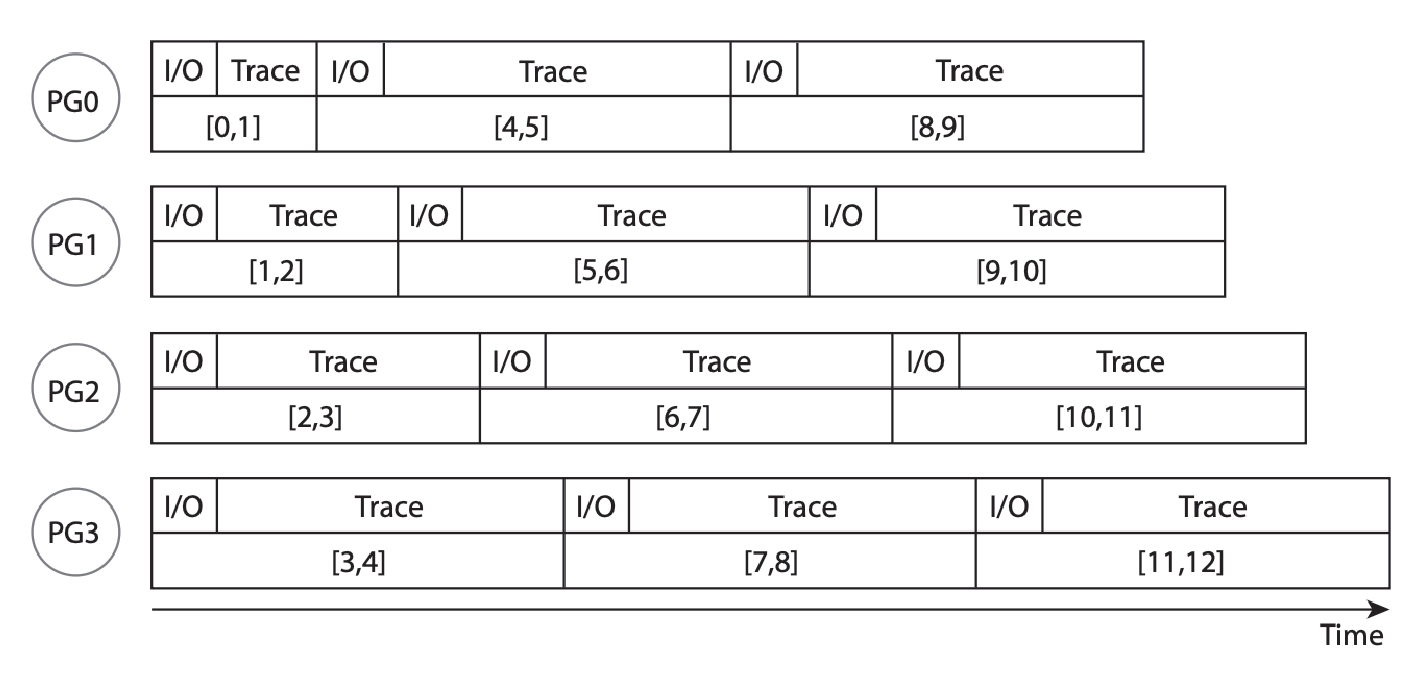
\includegraphics[width=\linewidth,keepaspectratio]{image/loadbalance/Round-robin.eps}
  \caption{
    基于轮转法的数据重划分算法\parencite{NouanesengsyLLSP12}。
 }
\label{fig:loadbalance:round-robin}
\end{figure}

而为了更进一步地解决计算负载不平衡的瓶颈,
研究者也使用了负载感知方法\parencite{NouanesengsyLS11},静态评估每个数据块的负载,并据此对数据块进行分配。该方法需要通过一个预处理阶段得到数据块之间的访问依赖关系,再结合初始粒子的数量和分布去预估每个数据块的负载,然后使用划分算法进行划分。该方法将数据块的划分看作可重叠的划分任务,每一个进程每轮被分配数据块的同样的一定占比,即处理该数据块中一定比例的粒子,进行逐块(Block-wise)的粒子追踪。该优化的任务目标是最小化粒子追踪整个过程中多个进程之间的负载差异之和。该方法最终采用参数最优化的解析计算方式,计算得出每一个数据块分配给各个进程的占比参数,并据此为划分策略进行数据块的划分。每个进程只负责重复数据块中一部分的粒子追踪的工作量,但总的负载比较均等。不过,由于需要比较复杂的预处理过程,该方法只适合于种子数量很多的情况,种子数量比较少时并不划算。此外,该负载静态评估的方法也需要提前知道初始粒子的分布。
图\ref{fig:loadbalance:static_partition}给出了该工作的一个划分过程示意图。

\begin{figure}[!tb]
%\setlength{\abovecaptionskip}{0.05cm} 
%\setlength{\belowcaptionskip}{-0.20cm}
  \centering
  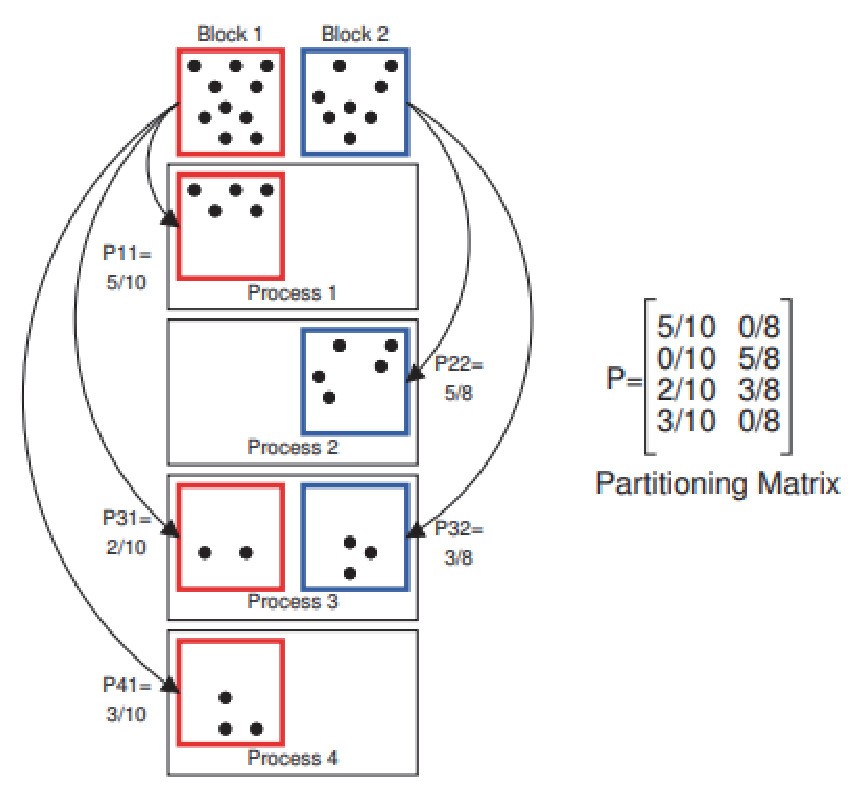
\includegraphics[width=.7\linewidth,keepaspectratio]{image/loadbalance/static_partition.eps}
  \caption{
    基于负载感知的静态数据重划分方法\parencite{NouanesengsyLS11}。
 }
\label{fig:loadbalance:static_partition}
\end{figure}

按照网格规则划分虽然操作比较简单,但是没有考虑流场数据本身的特点,是一种粗粒度的划分。对于一些特点非常明显的流场而言,基于这些流场特征的不规则划分往往更高效。如图所示,图\ref{fig:loadbalance:flowdirection}中小圆圈表示种子点,黑色实线表示流场的流向。红色虚线是按照网格规则划分的结果,这种划分方法会导致场线频繁地进入不同进程负责的数据块,造成额外的通信开销。不仅如此,按照图上的种子分布,粒子追踪过程中会有一部分进程经常处于空闲状态,造成负载不均衡的现象。因此,这时候我们往往需要考虑另一类数据划分方法,即不规则的数据划分。图\ref{fig:loadbalance:flowdirection}中蓝色虚线展示了一种根据流场方向的数据划分方法\parencite{ChenF08}。这种方法在划分的过程中考虑了种子的分布和诸如漩涡等流场的局部特征,在保证进程负载均衡的情况下,尽量使得每个粒子的追踪计算始终由同一个进程或很少的进程负责完成,减少了进程通信和同步带来的巨大开销。

\begin{figure}[!tb]
  \centering
  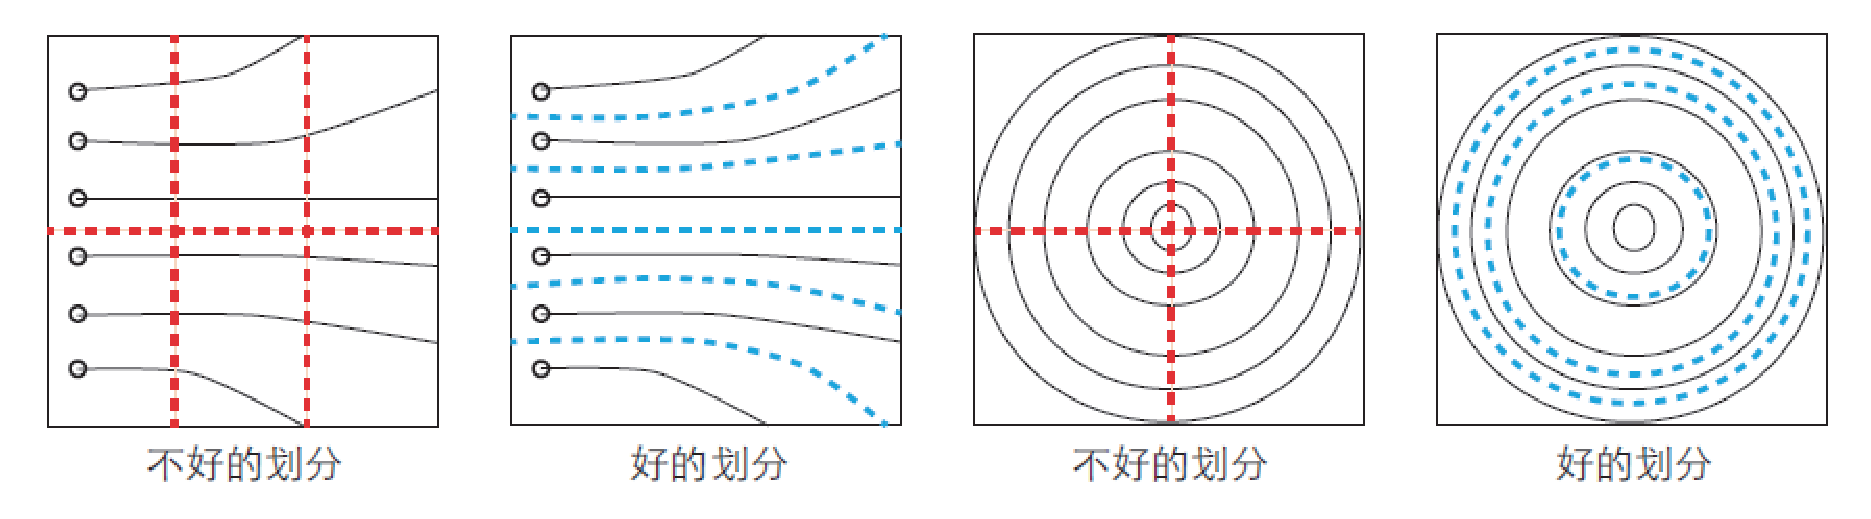
\includegraphics[width=.9\linewidth,keepaspectratio]{image/loadbalance/flowdirection.eps}
  \caption{
    规则划分和按照流场方向不规则划分的比较\parencite{ChenF08}。
 }
\label{fig:loadbalance:flowdirection}
\end{figure}

另一种不规则的划分是利用层次聚类进行自适应网格区域划分\parencite{YuWM07}。如图\ref{fig:loadbalance:hierarchical_partition}所示,数据首先被分解成单位网格,即最小的簇,然后具有类似模式的相邻网格会被两两合并,自下而上迭代地形成二叉树的层次结构。二叉树的深度实际上反映了流场特征的粒度。在数据划分时,可以根据该结构灵活选择不同层次中的簇(图中蓝点所示),评估其对应区域的负载,然后再分配给不同的进程。这两种不规则划分的方法都依赖于流场特征分析,但是在分布式环境中如何准确定义特征,也是一个新的挑战。而且,数据预处理和算法中需要预知粒子分布也带来了额外的计算负担。

\begin{figure}[!tb]
  \centering
  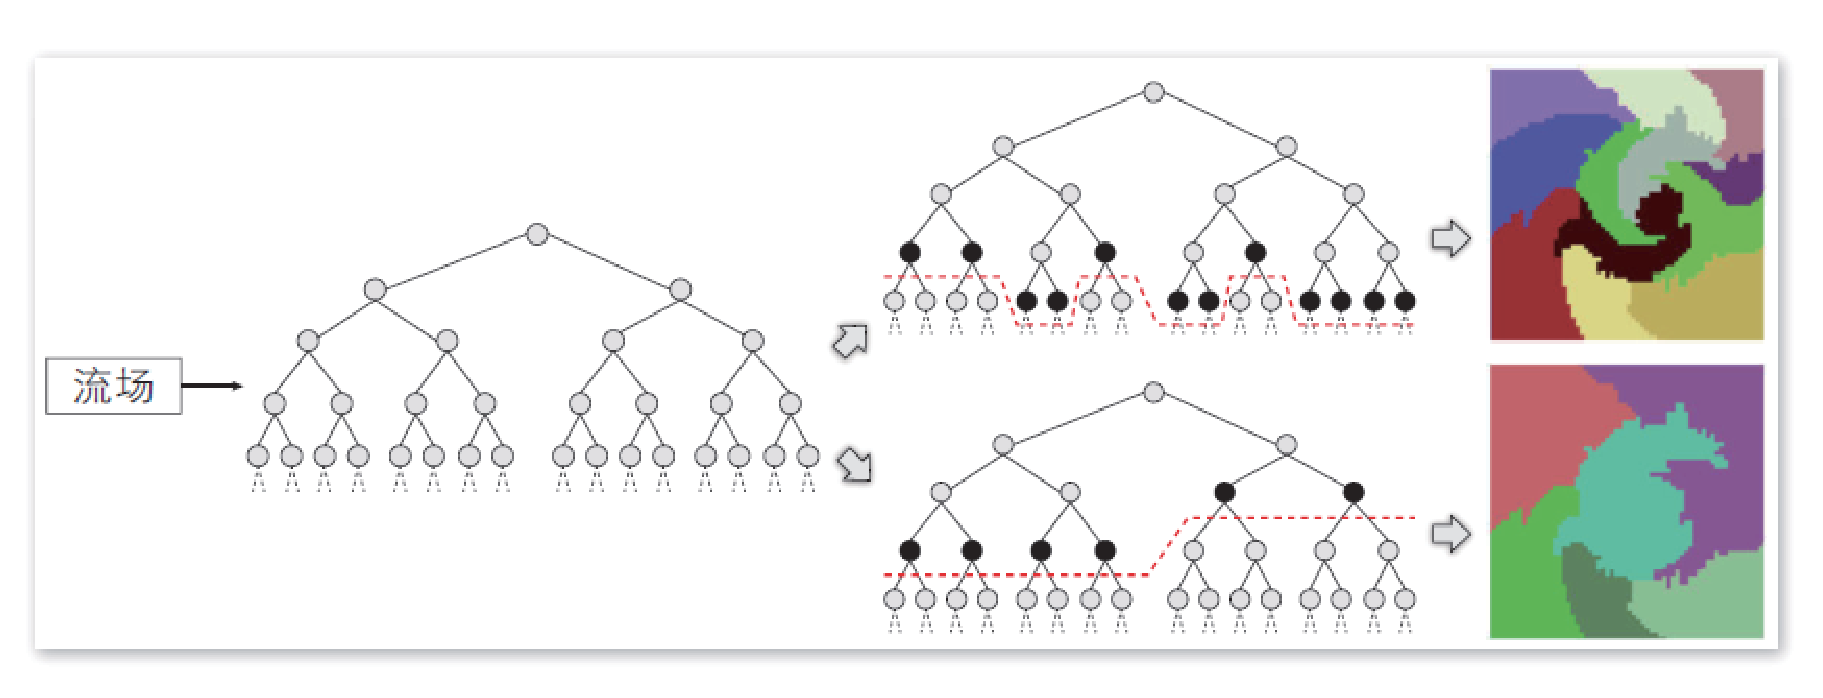
\includegraphics[width=\linewidth,keepaspectratio]{image/loadbalance/hierarchical_partition.eps}
  \caption{
    基于自适应层次聚类的数据划分\parencite{YuWM07}。
 }
\label{fig:loadbalance:hierarchical_partition}
\end{figure}

为了克服静态数据划分和分配的缺点,研究者们也提出了一些动态负载平衡的方 法。与静态方法相反,动态方法旨在粒子追踪过程中对数据进行动态划 分并将划分的数据块重新分配给各个进程,以达到负载平衡的目的。
数据重划分算法主要包含几何和拓扑两类。
几何方法根据划分对象的几何坐标进行划分,
包括递归坐标二分(recursive coordinate bisection, RCB)\parencite{BergerB87},
递归惯性二分(recursive inertial bisection, RIB)\parencite{Simon91},
以及空间填充曲线(space-filling curves)\parencite{PilkingtonB94}等算法,
而拓扑方法则需要先构造分区对象的拓扑结构,将其转化为图\parencite{GeorgeV96}
或者超图\parencite{CatalyurekBDBHR07}的结构再进行划分。
一般而言,拓扑方法精度更高,但比几何方法开销更大。
在该工作中,数据重划分本身的计算代价应当尽量小,
这样才能减轻对整体并行粒子追踪计算的性能的影响。
在数据重划分操作上花费过多的额外开销是不可取的。
因此,该方法在实现时采用了Zoltan并行数据服务工具包\parencite{DevineBHHV02}提供的
一种递归坐标二分(recursive coordinate bisection, RCB)的几何划分方法\parencite{BergerB87},
来解决公式中的优化问题。
RCB算法的思想如图\ref{fig:dynamicdr:repartition}(a)所示,其在Peterka等人之前的工作\parencite{PeterkaRNLSKH11}中也得到了应用。
在该算法中,每个数据块被看作一个划分单元,每个划分单元都有唯一的几何坐标,
并以对应数据块的预估负载为权重。

\begin{figure}[!tb]
%\setlength{\abovecaptionskip}{0.05cm} 
%\setlength{\belowcaptionskip}{-0.20cm}
  \centering
  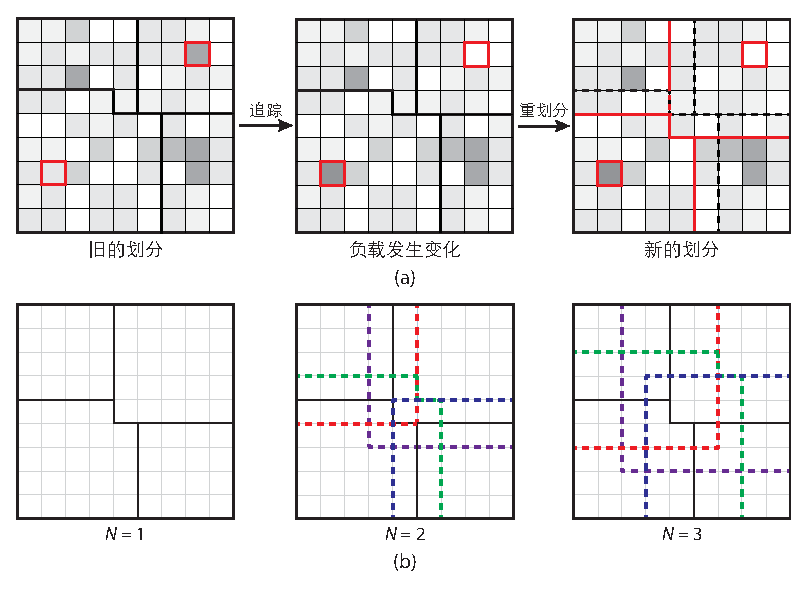
\includegraphics[width=.85\linewidth]{image/loadbalance/repartition.eps}
  \caption{
    动态数据重划分流程示例\parencite{ZhangGYP18}。
  }
  \label{fig:dynamicdr:repartition}
\end{figure}

北京大学可视化和可视分析小组提出了一种基于负载感知的数据重划分的方法\parencite{ZhangGYP18},可以动态地平衡并行粒子追踪过程中的负载,有效地了解决流场计算中的负载平衡问题。
相较于静态负载平衡方法,
这里所提出的方法在初始时使用一般的数据划分和分配策略,不会带来任何预处理开销。
运行时过程被管理为若干个轮次,其目的是平衡每一轮的粒子追踪计算。
在每一轮的追踪之前(除去第一轮),
算法会根据每个数据块的历史负载信息和其中未完成粒子的分布,
动态地评估该轮中每个数据块的负载。
基于负载评估的结果,算法可以执行数据重划分操作,
使得每个进程可以被重新划分和分配到一定的数据块,并继续下一轮的粒子追踪计算。

由于数据冲划分操作会造成一定的开销,
该方法通过适当增大每一轮中的负载,来减小数据重划分的频率。
该方法同时定义在每一轮中每个粒子可以穿过多个数据块,
在负载评估时统计粒子在所有这些数据块上的负载,用于随后的数据划分。
在这样的设定下,可能会出现同一轮中不在同一个起始数据块的粒子会经过相同的数据块的情况,
而这些粒子是可能会被分配给不同的进程的。
因此,为了保证划分后每个进程能够进行独立的粒子追踪,
该方法允许进程之间出现数据重叠。
为了达到这一目的,
该方法在运行时动态地建立了一个图模型,根据粒子的历史数据访问信息记录数据块之间的一阶访问依赖,
用于在负载评估过程中预测从一个数据块到另一个数据块的粒子转移数目,这一操作在每一轮追踪前对未完成粒子被执行。

基于数据重划分管理策略的动态负载平衡方法既可以被用到定常流场中用于计算流线,也可以被用在非定常流场中进行迹线计算。
对于定常流场中的流线计算,
数据只需要被所有进程按照初始划分策略一次性载入,并在数据重划分之后进行交换。
对于非定常流场中的迹线计算,
由于数据包含多个时间步,往往会超出内存的限制,
该方法将其划分为若干个时间步区间,并依次载入处理,使得每个时刻内存中只有一个时间步区间。
每个时间步区间实际上可以被视为具有相同时间维度的定常流场,
因此该方法可以使用和定常流场中的相同方式来处理其粒子追踪和数据重划分操作。

\begin{figure}[H]
%\setlength{\abovecaptionskip}{0.05cm} 
%\setlength{\belowcaptionskip}{-0.20cm}
  \centering
  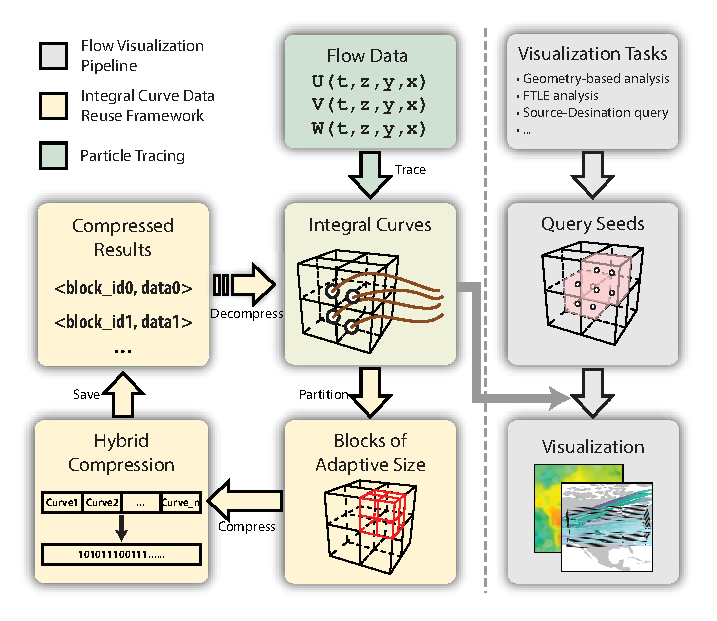
\includegraphics[width=\linewidth,keepaspectratio]{image/loadbalance/workflow.eps}
  \caption{
    并行粒子追踪计算框架的工作流程\parencite{ZhangGYP18}。
    从对原始数据的初始划分和分配开始,
    该方法通过一个多轮的过程对粒子进行追踪计算。
    在每一轮追踪结束后执行动态数据重划分操作,并按照新的数据分配方案继续下一轮的粒子追踪,
    直至所有粒子完成计算。
 }
\label{fig:dynamicdr:workflow}
\end{figure}

图\ref{fig:dynamicdr:workflow}给出了该方法中的并行粒子追踪计算框架。
给定初始的流场数据划分和粒子种子,
接着就可以开始并行粒子追踪计算。
追踪过程被管理为一个多轮的计算过程。
在每一轮追踪完成后,该方法对所有数据块在下一轮的负载进行动态评估,以此来重划分数据。
之后,算法按照重划分方案将数据和未完成粒子在进程间进行交换,并开始下一轮的粒子追踪计算。

在每一轮中,每个进程独立地进行粒子追踪计算。
为了确保每个进程能有相近的计算时间,每一轮进程的工作负载分布需要尽量均衡,
否则总会有一些进程在等待其他繁忙进程结束本轮计算,造成负载不平衡现象。
因此,如何保持每一轮的负载均衡是非常关键的,也是该方法进行动态数据重划分的目标。 

在每一轮粒子追踪计算完成后,如果还有未完成粒子,
该方法执行数据重划分操作,以期平衡随后的一轮中进程的负载。
具体来说,该方法通过动态地评估每个数据块中未完成粒子在下一轮中的负载,
之后通过对数据进行重划分将其重新分配给进程。
由于非定常流场可看作是多个不同时间步区间下的定常流场,
本文将在定常流场中进行数据重划分作为一般情况来对本章工作进行描述。

该方法同样使用粒子追踪的积分步数来衡量工作负载。
在每一轮中,数据块的负载被定义为所有粒子在该轮中在此数据块内被追踪的步数的总和。
由于每个进程对应一个数据划分,包含了若干数据块,因此其负载也是这些数据块的负载之和。
该方法需要评估每一轮中每个数据块的负载(第一轮除外),
从而可以根据评估结果使用数据重划分方法平衡各个进程的负载。

该工作同时将粒子数目和其历史负载进行考虑,用于预估数据块在每一轮中的负载。
在运行时该方法记录在每个数据块中追踪过的粒子数目和积分步数,并将其作为历史追踪信息附加在这个数据块中。
当一轮粒子追踪结束时,
该方法可以计算每个数据块中粒子的平均负载。
同时,根据未完成粒子的坐标,该方法同时可以获知它们接下来在所有数据块中的分布数量。
因此,每个数据块在下一轮的负载可以用如下方法评估得到。
假设在第$j-1$轮追踪结束之后,算法希望评估第$j$轮的负载。
对于每一个数据块$k$,如果在第$j$轮有$n_{k,j}$个粒子以它为起始块,
那么其预估负载可以使用如下公式进行计算:
\begin{equation}
\label{equ:dynamicdr:estimate}
\begin{aligned}
\overline{w_{k,j}}(n_{k,j})\ =\ \frac{\sum\nolimits_{i=0}^{j-1}w_{k,i}}{\sum\nolimits_{i=0}^{j-1}n_{k,i}} \times n_{k,j},
\end{aligned}
\end{equation}
其中,$w_{k,i}$是数据块$k$在前面的第$i\ (i<j)$轮中的实际负载,
$n_{k,i}$是在前面的第$i\ (i<j)$轮中经过数据块$k$的实际粒子数目。

\begin{figure}[!tb]
%\setlength{\abovecaptionskip}{0.05cm} 
%\setlength{\belowcaptionskip}{-0.20cm}
  \centering
  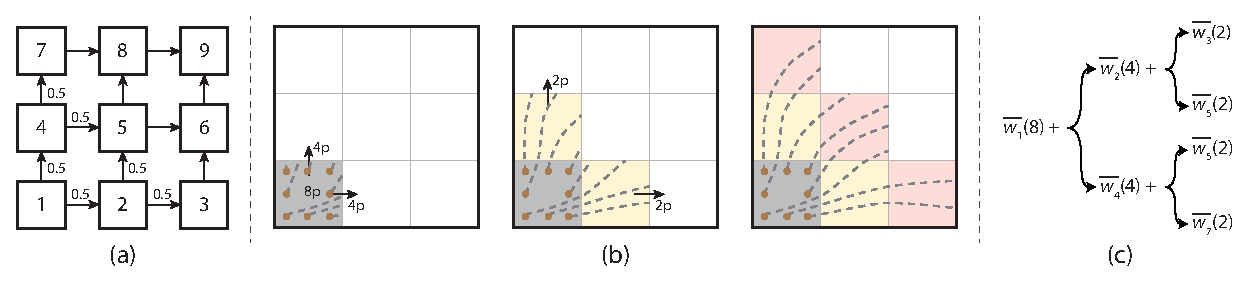
\includegraphics[width=\linewidth]{image/loadbalance/estimate.eps}
  \caption{
    基于ADG的负载评估二维示意图\parencite{ZhangGYP18}。
    (a)在运行时,该方法动态建立访问依赖图;
    (b)对于包含8个粒子的初始数据块1,
    该方法预测在每级追踪深度层次上可能访问的数据块以及粒子在这些数据块中的分布数量,
    这里面数据块之间的箭头表示对粒子下一步走向的预测(箭头边的数字表示粒子转移数量),
    棕色点表示初始粒子,由棕色点出发的虚线表示对粒子追踪情况进行的模拟;
    (c)初始数据块1的预估负载为这8个粒子在(b)中所有数据块中产生的负载的总和。
  }
  \label{fig:dynamicdr:estimate}
\end{figure}

该方法中规定了一个粒子在每轮可以穿过一定数量($N$个)的数据块。
在每一轮中,对于每一个数据块,%从一个数据块开始追踪的粒子,
算法应该评估从该数据块出发的粒子经过$N$个数据块所产生的负载。
当追踪深度$N=1$时,算法只需直接通过公式\ref{equ:dynamicdr:estimate}计算每个数据块的预估负载。
但是当追踪深度$N>1$时,
该方法则还需要知道从一个数据块开始的未完成粒子后面会经过哪些数据块,以及在这些数据块中产生的负载,
才能对这个数据块在这一轮的负载进行全面的评估。
为了达到这个目的,该方法在运行时动态地建立了一个一阶访问依赖图(access dependency graph, ADG)。
在以往的工作中,ADG已经被成功地应用到了有限资源下的流线和迹线计算中\parencite{ChenXLS12,ChenNLS12}。
需要注意的是,这里面该方法没有使用高阶访问依赖的方法,主要是因为高阶访问依赖的计算更为复杂,
而且占用更大的空间,对原本并行粒子追踪的效率影响更大。
在该工作中,每个数据块以多个\texttt{<key, value>}键值对的形式保有ADG的一部分,
其中\texttt{key}是该数据块的邻接块的索引,\texttt{value}是对应的访问转移概率。
在追踪过程中,每个进程计算其所负责的每个数据块关联的访问依赖。
在每一轮粒子追踪结束后,进程通过通信将其计算的ADG的一部分发送到所有其他进程,
使得每个进程都可以获得涵盖所有数据块的完整的ADG。
这种方法可以预测在随后的一轮中
未完成粒子会经过哪些数据块以及粒子在这些数据块中的分布数量。
因此,当追踪深度$N>1$时,根据从初始数据块的访问转移关系,
预测在第二级追踪深度层次上要访问的数据块得以实现。
基于访问转移概率,该方法同样可以预测粒子在这些数据块中的粒子分布数量。
之后,根据公式\ref{equ:dynamicdr:estimate}可以计算得到在每个数据块中的负载。
从这些数据块出发,该方法可以进一步预测在下一级追踪深度层次上要访问的数据块,
直至追踪到第$N$级追踪深度层次。
图\ref{fig:dynamicdr:estimate}展示了追踪深度为3时的负载评估示例。
该方法将初始数据块中的未完成粒子在这些所有涉及到的数据块中的负载累加,
即可得到该初始数据块的预估负载。

在动态负载评估之后,该方法根据对每个数据块的负载评估对数据进行重划分。
在此之前,该方法首先定义一个重划分模型来分析需要解决的问题。
在这个重划分模型中,每个数据块被看作是一个重划分的基本单元和对象,其预估负载被看作是这个对象的权重。

假设原始数据被划分成$m$个数据块,它们分别是$C = \{C_0, C_1, C_2, \cdots, C_{m-1}\}$,
在第$k$次数据重划分之前(即在进行了$k$轮的粒子追踪之后),
对这些数据块的预估负载分别为$w_{k} = \{w_{k,0}, w_{k,1}, w_{k,2}, \cdots, w_{k,m-1}\}$。
对于$n$个进程,算法需要将这些数据块划分为$n$个组,即$G = \{G_0, G_1, G_2, \cdots, G_{n-1}\}$,
其中$G_i = \{C_{i_0}, C_{i_1}, C_{i_2}, \cdots\}$。
每一组的负载是其所包含的所有数据块的负载之和:
$w_{k,{G_i}} = w_{k,{i_0}} + w_{k,{i_1}} + w_{k,{i_2}} + \cdots$。
为了达到负载均衡的目的,划分后的数据块组需要有近似相同的负载。
这里引出了一个最优化问题:最小化每两个数据块组之间的负载差异,即:
\begin{equation}
\label{eqt:dynamicdr:optimization}
\begin{aligned}
  \textrm{min}\ \mathcal{W}_k = \sum_{i=0}^{n-1}\left|w_{k,{G_i}} - \frac{1}{n}\sum_{j=0}^{n-1}w_{k,{G_j}}\right|.
\end{aligned}
\end{equation}

对于数据重划分,这个最优化问题也有一个限制条件。
为了减小重划分之后进程之间的数据交换,
新旧划分之间的重叠必须要尽可能大,也即是新的划分方案
相较于原来的划分方案不应该有显著的变动。

在该工作中,并行粒子追踪框架同时可以用于计算定常流场中的流线和非定常流场中的迹线。
上面描述的方法可以直接应用于定常流场数据。
对于非定常流场,数据块同时包含了空间和时间的维度。
该方法按照先后顺序载入和处理每个时间步区间的数据。
在一个时间步区间中,由于时间维度都是相同的,其数据可以看作是空间块,同时假定相邻时间步的数据具有一定的时间相关性。
对于每一个时间步区间,该方法建立一个新的ADG,并将其用于评估负载和执行数据重划分操作。
这一过程和在定常流场中的做法一致。
当一个时间步区间完成后,该方法根据上一次的重划分结果载入下一个时间步区间,当前的时间步区间则会从内存中清除。
使用这种方法,所有数据不必一次性读取,提高了内存效率。

在执行动态数据重划分时,该方法也使用了一些策略来提高计算的整体性能。
首先,算法适当减小了第一轮的粒子追踪步数。
第一轮只采用了一般的数据划分和分配方法,因此其负载平衡无法保证。
%因此当第一轮的负载比较大时,进程间负载失衡的可能性也在增加。
其次,当未完成粒子的总数比较小时,该方法不执行数据重划分操作。
数据重划分会导致数据在进程间的移动,带来额外的开销。
这种开销有可能会超过由数据重划分带来的性能增益,特别是在最后几轮剩余粒子数非常少的时候。在这种情况下,执行数据重划分操作并不划算。

总的来看,这些方法使用不同的策略,从不同方面一定程度上解决了数据管理方面的问题。
不过,它们在试图提高并行粒子追踪过程中的I/O效率和负载均衡性等影响性能的因素的同时,也带来了各种预处理和运行时过程中其他方面的耗费,
不可避免地会影响并行粒子追踪的整体性能和可扩展性。
从这一方面看,
大规模流场可视化数据管理还需要处理在提高并行粒子追踪性能的同时又会带来其他耗费这两者之间的矛盾。
如何平衡这两个方面的矛盾也是针对大规模流场可视化的数据管理需要考虑的问题。

\subsection{混合并行的流场可视化中的针对负载均衡问题的经典解决方案}
任务并行和数据并行方法在不同的角度上改善了并行粒子追踪的可扩展性,
但是它们在某些方面也都有各自的局限性。%,如表\ref{table:background:comparison}所示。
近年来,研究者们将这两种并行策略结合起来,
提出了混合并行的方法,以期能够进一步提高并行粒子追踪计算的性能。
 
 
\begin{figure}[!tb]
  \centering
  \includegraphics[width=1.0\linewidth]{image/loadbalance/dstep.eps}
  \caption{
    基于DStep框架的混合并行粒子追踪计算\parencite{KendallWAPHE11}。
  }
  \label{fig:background:dstep}
\end{figure}

DStep\parencite{KendallWAPHE11}是由Kendall等人提出的一种类似于
MapReduce\parencite{JeffreyS08}的框架,
可用于解决并行域遍历问题,包括并行粒子追踪的计算(如图\ref{fig:background:dstep}所示)。
DStep有效地结合了两种并行策略的优点:
在数据并行方面,使用轮转的方式静态划分数据;
在任务并行方面,使用基于专有任务队列的任务管理来完成不同类型的任务;
这些都使其进一步提高了并行粒子追踪的可扩展性。
此外,DStep在预处理和运行时都没有特殊的需求,因而非常适用于粒子追踪的并行计算。
研究表明,该框架在超过6万个BlueGene/P核的并行计算环境下仍然具有比较好的性能。
在该工作的基础上,北京大学可视化小组的Guo等人\parencite{GuoYHZ13}和Liu等人\parencite{LiuGZY16}继承了DStep框架并进行了重新设计,
用于在集合模拟数据中生成和管理大规模的迹线,
使系统能够在有限的内存资源环境下运行,同时可以平衡吞吐率和负载均衡之间的关系。
随后,为了将拉格朗日属性空间的投影引入到多变量流场数据的分析上,
Guo等人\parencite{GuoHSZHY14}还进一步改进了DStep框架,
将其与Pivot MDS投影算法\parencite{BrandesP06}集成,
可以支持大规模的并行迹线计算和分析。
这些工作都获得了很好的可扩展性。

混合并行方法充分结合了任务并行和数据并行的优势,能够克服两者固有的一些缺点。
混合并行不需要任何的预处理分析。
由于增加了设计和实现上的复杂性,针对粒子追踪计算的混合并行方法也给研究人员提出了更高的要求。
不过,针对一些特定应用
我们可以充分利用所要解决问题的性质,研究合适的混合并行计算策略。

\subsection{小结}
该小节针对当下大规模科学数据的分析探索中采用的并行计算框架内部中的负载均衡问题做出了深刻的分析和探讨,论述了负载均衡问题对于并行计算的重要性。针对大规模流场可视化中存在的问题,该部分进一步明确了并行粒子追踪任务过程中,具体的负载均衡问题产生的原因和本质,并据此提出了基于动态负载评估和基于K-D树划分的两种改善并行粒子追踪过程中负载不平衡问题的行之有效的解决策略。负载均衡问题是大规模科学数据中采用并行计算手段
中的核心问题,对其诊断和改良因而具有十分重要的意义,是大规模数据管理策略中不可缺少的重要组成部分。

